\documentclass[18pt, oneside]{article}   	
\usepackage{geometry}                		
\geometry{letterpaper}                   		 
%\geometry{landscape}                		
%\usepackage[parfill]{parskip}    		
\usepackage{graphicx}				
\usepackage{tikz}										
\usetikzlibrary{shapes.misc}
\usetikzlibrary{backgrounds}
\tikzset{cross/.style={cross out, draw=black, minimum size=2*(#1-\pgflinewidth), inner sep=0pt, outer sep=0pt},
%default radius will be 1pt. 
cross/.default={1pt}}

\usepackage{amssymb}
\setlength{\parindent}{0pt}
\title{Lecture Note Second Portion} 
\author{Jody Shu}
%\date{}							

\begin{document}
\maketitle
%\section{}
%\subsection{}
\begin{Large}
\textbf{Q}: What if the data is not linear separable?

\vspace*{1cm}\hspace{6cm}%
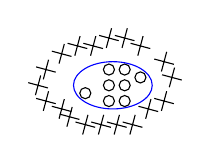
\begin{tikzpicture}[]



\draw (7,5) circle (2pt);
\draw (7,5.2) circle (2pt);
\draw (7,5.4) circle (2pt);
\draw (6.8,5) circle (2pt);
\draw (6.8,5.2) circle (2pt);
\draw (6.8,5.4) circle (2pt);
\draw (6.5,5.1) circle (2pt);
\draw (7.2,5.3) circle (2pt);

\draw (7.5,5) node[cross=3pt,rotate=30] {};
\draw (7.6,5.3) node[cross=3pt,rotate=30] {};
\draw (7.5,5.5) node[cross=3pt,rotate=30] {};

\draw (7.3,4.9) node[cross=3pt,rotate=30] {};
\draw (7.1,4.7) node[cross=3pt,rotate=30] {};
\draw (6.9,4.7) node[cross=3pt,rotate=30] {};
\draw (6.7,4.7) node[cross=3pt,rotate=30] {};
\draw (6.5,4.7) node[cross=3pt,rotate=30] {};
\draw (6.3,4.8) node[cross=3pt,rotate=30] {};
\draw (6.2,4.9) node[cross=3pt,rotate=30] {};
\draw (6.,5) node[cross=3pt,rotate=30] {};
\draw (5.9,5.2) node[cross=3pt,rotate=30] {};
\draw (6.,5.4) node[cross=3pt,rotate=30] {};
\draw (6.2,5.6) node[cross=3pt,rotate=30] {};
\draw (6.4,5.7) node[cross=3pt,rotate=30] {};
\draw (6.6,5.7) node[cross=3pt,rotate=30] {};
\draw (6.8,5.8) node[cross=3pt,rotate=30] {};
\draw (7,5.8) node[cross=3pt,rotate=30] {};
\draw (7.2,5.7) node[cross=3pt,rotate=30] {};
\draw[ color=blue] (6.85,5.2) ellipse (0.5 and .3);
\end{tikzpicture}
\\
\textbf{Ans}: Use Kernel method

\end{Large}
\end{document}